\section{Manufacturing}
\subsection{Circuit Design}
A modular approach was used to construct the required circuit. Each of the components are tested individually before bringing them together. The circuit is shown as follows:

\begin{figure}
    \centering
    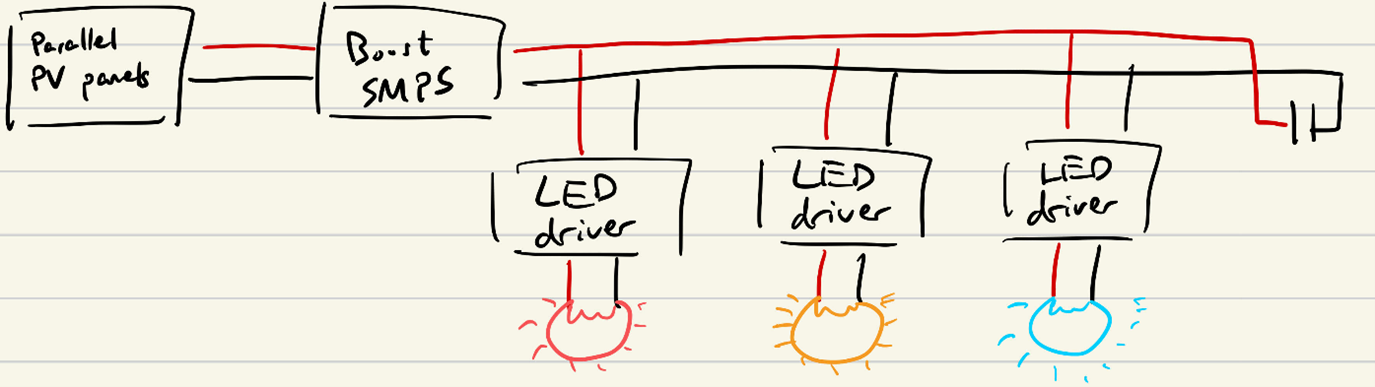
\includegraphics[width=0.8\linewidth]{images/circuit-design.png}
    \caption{}
\end{figure}

The power supply is chosen to be 3 parallel PV panels since only this configuration gives enough current. The power supply for series PV panels is too unstable to be implemented well in the design.

Two types of controller design are considered for the LED drivers. The first one is a simple controller that sets the duty cycle according to the amount of current through the SMPS. The second one is a PID controller. The advantage of a PID controller is that it provides better control and voltage regulation on the output. Although the result looks the same from both controllers, PID controller will be used since it gives better control over the output by the user.

Unfortunately, the bi-directional SMPS is absent at the time and during the demo, it will not be implemented in the final circuit design. In theory, it should control the supercapacitor for charging or discharging relative to the voltage in the DC grid.

Although this result is far from the ideal circuit, this circuit will be used in the demo since this circuit is easy to implement. Further amendments and improvements are mentioned in the evaluation subsection under power system.

\subsection{Chassis Design}

Many different design concepts were considered when it came to designing the chassis. 

% Chassis first draft
\begin{figure}
    \centering
    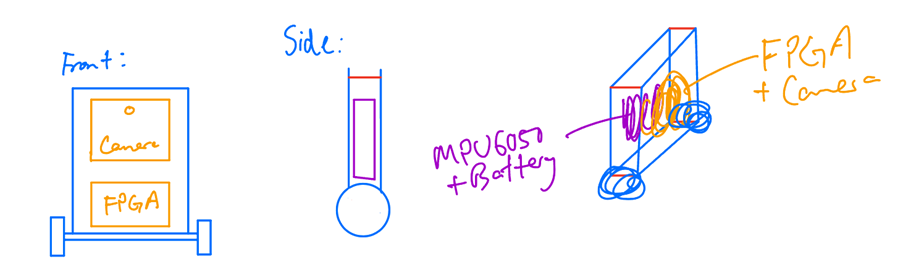
\includegraphics[width=0.8\linewidth]{images/chassis-drawing1.png}
    \caption{}
\end{figure}

This would be the simplest to build since it would only require one swivel wheel and not many changes are required to the existing chassis; just to make the wheels perfectly in the centre. However, it would be challenging to fit everything in such a tight narrow space widthout greatly widening the chassis. This would further prove to me even more difficult when it comes to debugging.

%roomba design
\begin{figure}
    \centering
    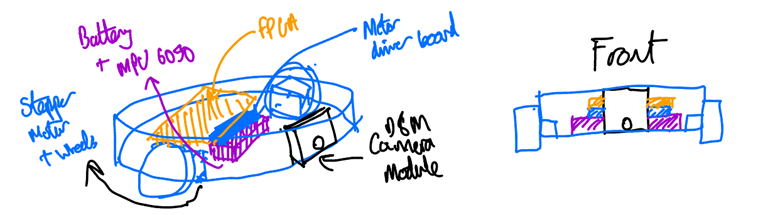
\includegraphics[width=0.8\linewidth]{images/chassis-drawing2.png}
    \caption{}
\end{figure}

This design resembles that of an automatic vacuum and has the most aesthetic look if made correctly. It provides enough space for all components to fit appropriately. With a design with the centre of mass super close to the wheels and ground, the control system cannot be easily implemented all ends could easily touch the ground. This is further supported by the fact that there is virtually no height meaning very little to no inertia at the top. This would mean the gyroscope would have a hard time detecting changes in angle tilt. Furthermore, a circular design would prove to be impractical when it came to driving around on the field.

\vspace{1cm}

%triple tower design
\begin{wrapfigure}{l}{0.4\linewidth}
    \centering
    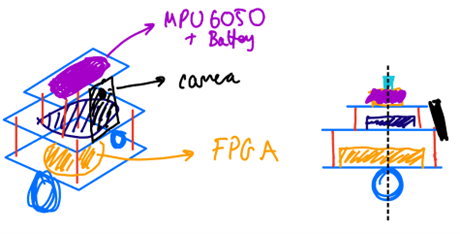
\includegraphics[width=\linewidth]{images/chassis-drawing3.png}
    \caption{}
\end{wrapfigure}

In the end, the triple tower design set up was chosen. This allowed a variable weight distribution via the use of nuts and threaded rods. This meant that when it came to testing, it was very convenient for us to change the heights of relevant parts to allow for an ideal control system. Making the tower very top heavy, resembled that of the heavy mass in an inverted pendulum. This modular design would ultimately save time and allow for a range of possibilities. Furthermore, this design would allow for quick and easy debugging without dismantling the whole system. 

M10 threaded rods were chosen to ensure that the chassis is rigid, robust and durable. This added plenty of mass to the rover. However, the fact that this mass was static meant that it added unnecessary weight. In turn, this meant that the torque produced by the wheels was insufficient, and as a result, bigger wheels would need to be printed to allow for further leverage. In hindsight, thinner threaded rods, and nuts of size maximum M5 would have been more than enough to keep the whole segway secure. This would have further saved time in 3d-printing our own wheels as the torque produced would have been sufficient since a small weight component means a smaller force as according to Newton’s second law.

The required torque can be calculated with the formula in figure \ref{formula:torque}

\begin{figure}
    \centering
    \(\text{Torque} = \text{height} \times \text{mass} \times \text{acceleration due to gravity} \times \sin (\text{maximum tilt})\)
    \caption{Torque Formula}
    \label{formula:torque}
\end{figure}
Using this formula, it is known that a vague minimum torque required. From this, it is needed to ensure that the maximum torque is below 0.96Nm. This value considers both stepper motors where the nominal value of 0.48Nm is taken from the datasheet. 

Therefore, as a next step, by reducing the mass diameter from M10 to M5, 75\verb|%| of the mass of the threaded rods would be eliminated. This means that the torque produced by the motors would be enough to take full advantage of the control system allowing for smooth operation. 

\begin{figure}
    \centering
    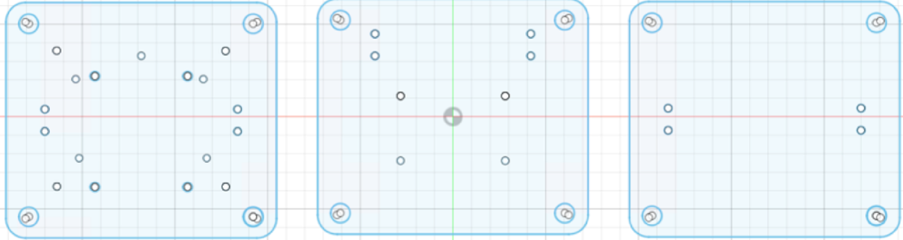
\includegraphics[width=0.8\linewidth]{images/chassis-cad1.png}
    \caption{}
\end{figure}

Fusion 360 was used to design the new chassis. A few changes were made based on the original design that was offered to make it better fit our requirements. Notably, the original wheel mounts were placed further apart were placed horizontally further apart with an offset in the Y-axis to allow for the wheels pivot to be in line with the centre of mass. 

Having the battery on top was chosen to allow it to be "top heavy" referring to a configuration in an inverted pendulum design in which most of the mass is concentrated at the top, increasing the pendulum's potential to tip over. This imbalance has an impact on the system's stability, requiring precise control to keep the system upright. This design largely relies on inertia, which is the resistance of an object to changes in motion. It is more difficult to quickly adjust the pendulum's position due to the top-heavy configuration's high inertia, which derives from the concentrated mass at the top. As a result, strong control measures are required to stabilise the system and reduce its consequences.

\begin{figure}
    \centering
    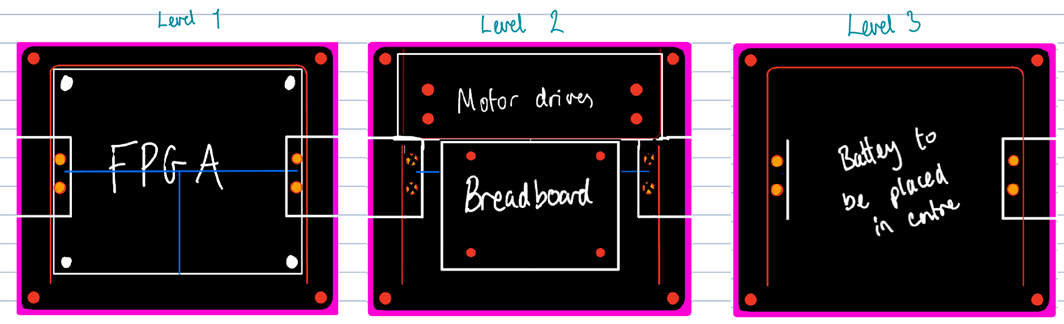
\includegraphics[width=0.8\linewidth]{images/chassis-cad2.png}
    \caption{}
\end{figure}

Combining all the levels gave us the following:

% complete chassis

\begin{figure}
    \centering
    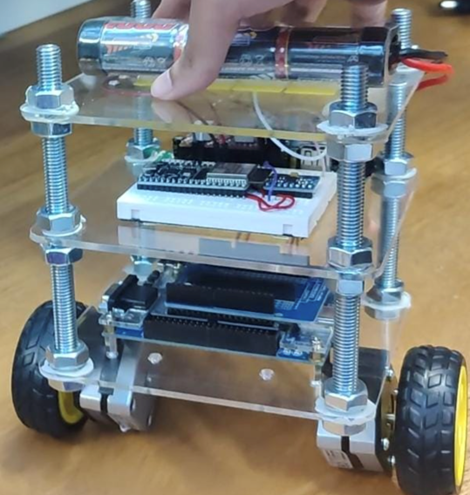
\includegraphics[width=0.8\linewidth]{images/final-chassis.png}
    \caption{}
\end{figure}